\documentclass{beamer}
\usepackage[utf8]{inputenc}
\usepackage[T1]{fontenc}
\usepackage[ngerman]{babel}
\usepackage{ae}
\usepackage{array}
\usepackage{tabularx}
\usepackage{graphicx}
\usepackage{amsmath}
\usepackage{textcomp}
\usepackage{blindtext}
\usepackage{listings}
\usepackage{booktabs}
\usepackage{icomma}

%Settings
\usepackage{icomma}

%Beamer Einstellungen
\usetheme{Goettingen}
\newcounter{chapter}

\setbeamertemplate{section in head/foot}{\hfill\thechapter.\insertsectionheadnumber.~\insertsectionhead}
\setbeamertemplate{section in head/foot shaded}{\color{structure!50}\hfill\thechapter.\insertsectionheadnumber.~\insertsectionhead}
\setbeamertemplate{section in toc}{\large\thechapter.\inserttocsectionnumber~\inserttocsection}
\makeatletter
\setbeamertemplate{section in sidebar}%{sidebar theme}
{%
  \vbox{%
    \vskip1ex%
    \beamer@sidebarformat{3pt}{section in sidebar}{\thechapter.\insertsectionheadnumber
~\insertsectionhead}%
  }%
}
\setbeamertemplate{section in sidebar shaded}%{sidebar theme}
{%
  \vbox{%
    \vskip1ex%
    \beamer@sidebarformat{3pt}{section in sidebar shaded}{\thechapter.\insertsectionheadnumber
~\insertsectionhead}%
  }%
}
\addtobeamertemplate{navigation symbols}{%
	\usebeamerfont{footline}%
 	\usebeamercolor[fg]{footline}%
 	\raisebox{.25ex}{\insertframenumber/\inserttotalframenumber}
}{}
\makeatother

%Farbe
\definecolor{mygreen}{rgb}{0,0.6,0}
\definecolor{mygray}{rgb}{0.5,0.5,0.5}
\definecolor{mymauve}{rgb}{0.58,0,0.82}
\definecolor{mybygrey}{gray}{.93}
\definecolor{eclipse-comments}{rgb}{0,0.6,0}
\definecolor{eclipse-strings}{rgb}{1,0,1}
\definecolor{eclipse-keywords}{rgb}{0,0,1}

% Lenghts
\setlength{\parskip}{.5\baselineskip plus .2\baselineskip minus .1\baselineskip}

%Eurozeichen
\usepackage{eurosym}
\DeclareUnicodeCharacter{20AC}{\euro}

%tabellen
\newcolumntype{L}{>{\raggedright\arraybackslash}X}

%Listings Ilog-Script-Definition
\lstdefinelanguage{IlogScript}{
  keywords=[1]{typeof, new, true, false, catch, function, return, null, catch, switch, var, if, in, while, do, else, case, break, for},
  keywordstyle=[1]\color{orange}\bfseries,
  keywords=[2]{class, export, boolean, throw, implements, import, this, execute, int, main},
  keywordstyle=[2]\color{blue}\bfseries,
  keywords=[3]{write, writeln, thisOplModel, cplex},
  keywordstyle=[3]\color{RedViolet}\bfseries,
  identifierstyle=\color{black},
  sensitive=false,
  comment=[l][\color{eclipse-comments}]{//},%
  morecomment=[s]{/*}{*/},
  commentstyle=\color{purple}\ttfamily,
  stringstyle=\color{mymauve}\ttfamily,
  morestring=[b]',
  morestring=[b]",
  showstringspaces=false
}[keywords,comments,strings]%

%Listings OPL Definition
\lstdefinelanguage[]{opl}%
{
  keywords=[1]{
    maximize, minimize, subject, to, forall, sum, solve, string, dvar, boolean, int, int+, float, float+, enum, tupel, ftoi, mod, abs, maxint, sqrt, ceil, floor, distToInt, frac, trunc, infinity, first, last, card, ord, next, prev, range, in, struct, prod, min, max, union, inter, not, initialize, var, dmin, dmax, dsize, bound, dnexthigher, alldifferent, circuit, distribute, try, endtry, tryall, if, endif, then, else, while, select, once, search, when, onValue, generate, generationMin, generationMax, generateSeq
  },
  keywordstyle=[1]\color{eclipse-keywords},
  morekeywords={..,=,<,>,<=,=>,==},
  keywords=[2]{typeof, new, true, false, catch, function, return, null, catch, switch, var, if, in, while, do, else, case, break},
  keywordstyle=[2]\color{orange}\bfseries,
  keywords=[3]{write, writeln, thisOplModel, from, DBConnection, DBRead, DBUpdate, SheetConnection, SheetRead, SheetWrite},
  keywordstyle=[3]\color{RedViolet}\bfseries,
  comment=[l][\color{eclipse-comments}]{//},%
  morecomment=[s][\color{eclipse-comments}]{/*}{*/},%
  string=[b][\color{eclipse-strings}]\``,%
  stringstyle=\color{mymauve}\ttfamily,
  morestring=[b]",%
  morestring=[b]',%
  showstringspaces=false
}[keywords,comments,strings]%

\lstset{ %
  backgroundcolor=\color{mybygrey},   % choose the background color; you must add \usepackage{color} or \usepackage{xcolor}
  basicstyle=\footnotesize\ttfamily,
  captionpos=b,                    % sets the caption-position to bottom
  commentstyle=\color{mygreen},    % comment style
  %deletekeywords={...},            % if you want to delete keywords from the given language
  escapeinside={\%*}{*)},          % if you want to add LaTeX within your code
  frame=leftline,                    % adds a frame around the code
  keywordstyle=\color{blue},       % keyword style
  language=opl,                 % the language of the code
  linewidth=\textwidth,
  morekeywords={*,documentclass,begin,title,author,date,maketitle},            % if you want to add more keywords to the set
  numbers=left,                    % where to put the line-numbers; possible values are (none, left, right)
  numbersep=5pt,                   % how far the line-numbers are from the code
  numberstyle=\tiny\color{mygray}, % the style that is used for the line-numbers
  rulecolor=\color{black},         % if not set, the frame-color may be changed on line-breaks within not-black text (e.g. comments (green here))
  stepnumber=1,                    % the step between two line-numbers. If it's 1, each line will be numbered
  stringstyle=\color{mymauve},     % string literal style
  tabsize=2,                       % sets default tabsize to 2 spaces
  xleftmargin=.05\textwidth,
  literate=%
    {Ö}{{\"O}}1
    {Ä}{{\"A}}1
    {Ü}{{\"U}}1
    {ß}{{\ss}}1
    {ü}{{\"u}}1
    {ä}{{\"a}}1
    {ö}{{\"o}}1
    {~}{{\textasciitilde}}1,
  title=\lstname                   % show the filename of files included with \lstinputlisting; also try caption instead of title
}

%Listings OPL Data Definition
\lstdefinelanguage[]{opldata}%
{
  keywords=[1]{
    maximize, minimize, subject, forall, sum, solve, string, dvar, boolean, int, int+, float, float+, enum, tupel, ftoi, mod, abs, maxint, sqrt, ceil, floor, distToInt, frac, trunc, infinity, first, last, card, ord, next, prev, range, in, struct, prod, min, max, union, inter, not, initialize, var, dmin, dmax, dsize, bound, dnexthigher, alldifferent, circuit, distribute, try, endtry, tryall, if, endif, then, else, while, select, once, search, when, onValue, generate, generationMin, generationMax, generateSeq
  },
  keywordstyle=[1]\color{eclipse-keywords},
  morekeywords={..,=,<,>,<=,=>,==},
  keywords=[2]{typeof, new, true, false, catch, function, return, null, catch, switch, var, if, in, while, do, else, case, break},
  keywordstyle=[2]\color{orange}\bfseries,
  keywords=[3]{write, writeln, thisOplModel, from, to, DBConnection, DBRead, DBUpdate, SheetConnection, SheetRead, SheetWrite},
  keywordstyle=[3]\color{RedViolet}\bfseries,
  comment=[l][\color{eclipse-comments}]{//},%
  morecomment=[s][\color{eclipse-comments}]{/*}{*/},%
  string=[b][\color{eclipse-strings}]\``,%
  stringstyle=\color{mymauve}\ttfamily,
  morestring=[b]",%
  morestring=[b]',%
  showstringspaces=false
}[keywords,comments,strings]%

\lstset{ %
  backgroundcolor=\color{mybygrey},   % choose the background color; you must add \usepackage{color} or \usepackage{xcolor}
  basicstyle=\footnotesize\ttfamily,
  captionpos=b,                    % sets the caption-position to bottom
  commentstyle=\color{mygreen},    % comment style
  %deletekeywords={...},            % if you want to delete keywords from the given language
  escapeinside={\%*}{*)},          % if you want to add LaTeX within your code
  frame=leftline,                    % adds a frame around the code
  keywordstyle=\color{blue},       % keyword style
  language=opl,                 % the language of the code
  linewidth=\textwidth,
  morekeywords={*,documentclass,begin,title,author,date,maketitle},            % if you want to add more keywords to the set
  numbers=left,                    % where to put the line-numbers; possible values are (none, left, right)
  numbersep=5pt,                   % how far the line-numbers are from the code
  numberstyle=\tiny\color{mygray}, % the style that is used for the line-numbers
  rulecolor=\color{black},         % if not set, the frame-color may be changed on line-breaks within not-black text (e.g. comments (green here))
  stepnumber=1,                    % the step between two line-numbers. If it's 1, each line will be numbered
  stringstyle=\color{mymauve},     % string literal style
  tabsize=2,                       % sets default tabsize to 2 spaces
  xleftmargin=.05\textwidth,
  literate=%
    {Ö}{{\"O}}1
    {Ä}{{\"A}}1
    {Ü}{{\"U}}1
    {ß}{{\ss}}1
    {ü}{{\"u}}1
    {ä}{{\"a}}1
    {ö}{{\"o}}1
    {~}{{\textasciitilde}}1,
  title=\lstname                   % show the filename of files included with \lstinputlisting; also try caption instead of title
}

% Makros
\RequirePackage{ifthen}
\newcommand{\sectionframe}[2][\empty]{
  \ifthenelse{\equal{#1}{\empty}}
    {\section{#2}}
    {\section[#1]{#2}}
  \begin{frame}
   \begin{center}
    \LARGE\bfseries \thechapter.\thesection{} #2
   \end{center}
  \end{frame}
}

\newcommand{\subsectionframe}[2][\empty]{
  \ifthenelse{\equal{#1}{\empty}}
    {\subsection{#2}}
    {\subsection[#1]{#2}}
  \begin{frame}
   \begin{center}
    \Large\bfseries #2
   \end{center}
  \end{frame}
}



%Always load hyperref last...
\usepackage{hyperref}


\begin{document}

\setcounter{chapter}{6}
\author[CC-BY-SA A.~Popp]{Andreas Popp\vspace{-2\baselineskip}}
\date[CC-BY-SA]{\begin{center}
                 
\includegraphics[width=.2\linewidth]{Icons/CCBYSAbig}
                \end{center}
\footnotesize Dieser Foliensatz ist lizenziert unter einer  \href{http://creativecommons.org/licenses/by-sa/4.0/}{Creative Commons Namensnennung - Weitergabe unter gleichen Bedingungen 4.0 International Lizenz}.}
\title[\thechapter{} Einfache techniken der stochastischen Optimierung]{\textbf{Modellierung und Optimierung mit OPL}\newline \thechapter{} Einfache techniken der stochastischen Optimierung}

\frame{\titlepage}


\begin{frame}[squeeze]
 \frametitle{Inhalt}\scriptsize
  \tableofcontents
\end{frame}

\begin{frame}
 \frametitle{Example: Vindoo Support}
 \begin{figure}
  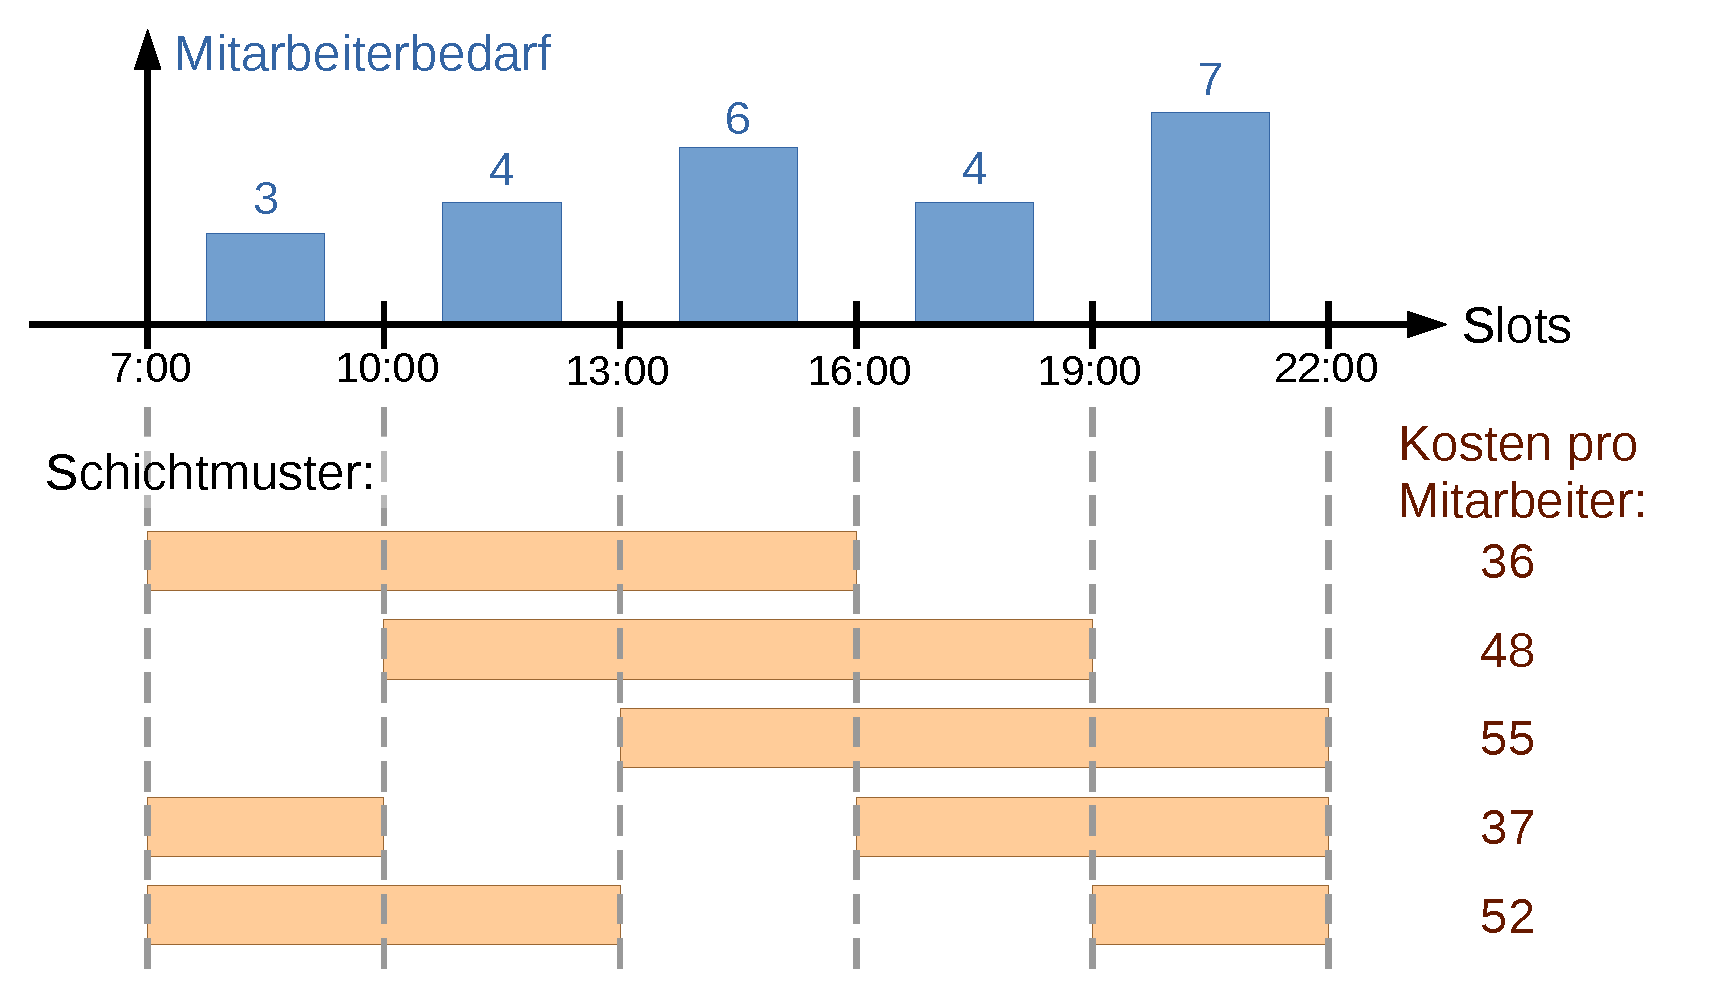
\includegraphics[width=\linewidth]{Bilder/Vindoo}
 \end{figure}
 {\footnotesize(cf. Pinedo: Planning and Scheduling in Manufacturing and Services)}
\end{frame}

\begin{frame}
 \frametitle{Model: Cyclic staffing problem}
 \begin{tabularx}{\linewidth}{lL}
  \multicolumn{2}{l}{\textbf{index sets}:}\\
     $T$ & set of time slots\\
     $S$ & set of shift patterns\\
  \multicolumn{2}{l}{\textbf{parameters}:}\\
     $c_s$ & cost per employee in shift pattern~$s\in S$\\
     $d_t$ & requirement of employees in shift pattern~$t\in T$\\
     $a_{ts}$ & Availability of employees in shift pattern~$s\in S$ in time slot~$t\in T$\\
  \multicolumn{2}{l}{\textbf{decision variables}:}\\
     $x_s$ & deployed employees in shift pattern~$s\in S$\\[1ex]
  \multicolumn{2}{l}{\textbf{model description}:}\\[1ex]
  \multicolumn{2}{l}{
      $
      \begin{array}{rllr}
	\min & \multicolumn{3}{l}{
		  \displaystyle\sum_{s\in S}c_s\cdot x_s
		}\\[3ex]
	s.t. & \displaystyle\sum_{s\in S} a_{ts}\cdot x_s \geq d_t & \quad\forall t\in T  & \mathrm{(I)}\\[.8ex]
	      & x_s \in\mathbb{Z}_0^+ & \quad\forall s\in S &\\
      \end{array}
      $
  }\\[1ex]
 \end{tabularx}
\end{frame}

\sectionframe[Optimization routine in OPL]{Optimization routine in OPL}
\begin{frame}
 \frametitle{Optimization routine in OPL}
 \begin{figure}
   \centering
   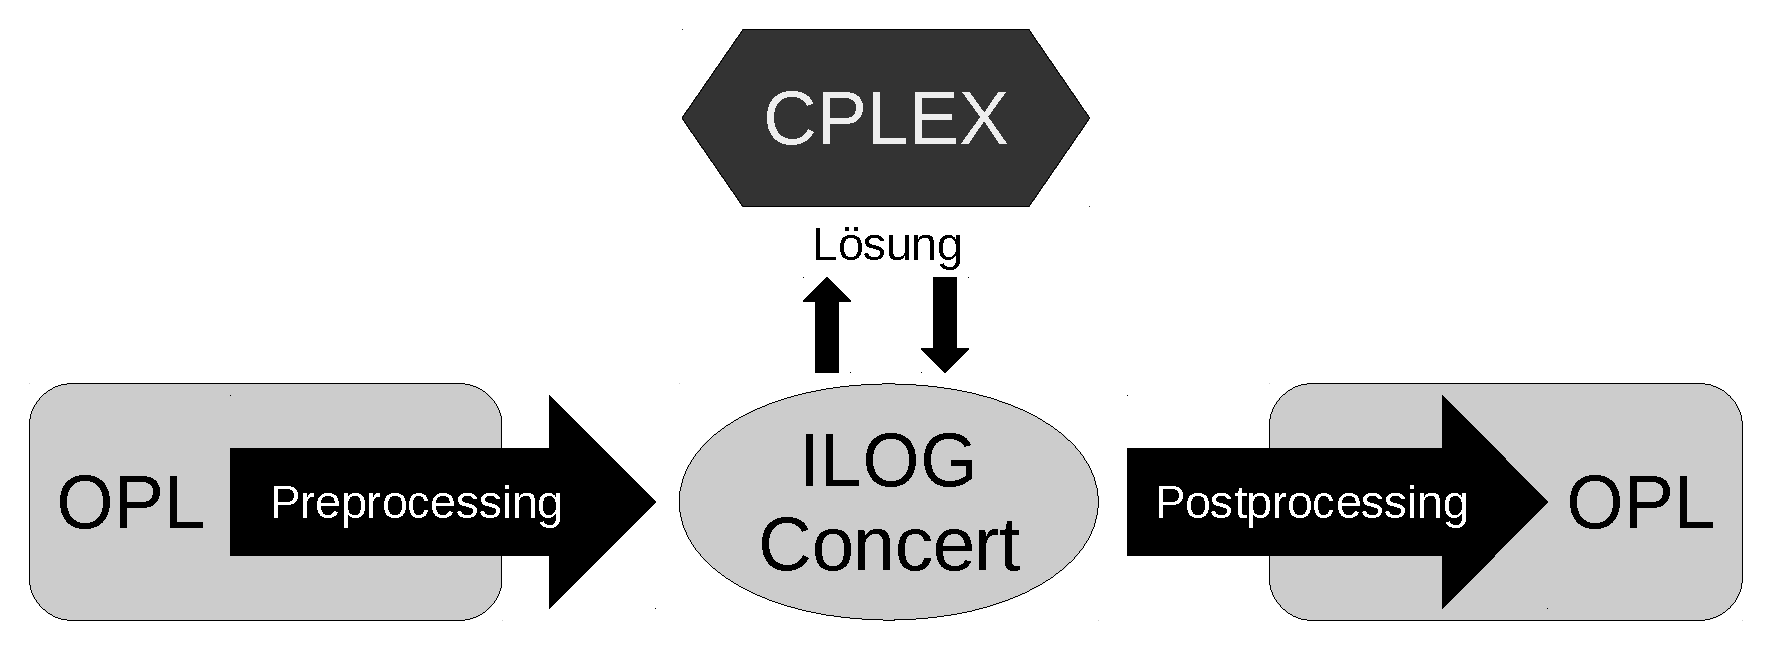
\includegraphics[width=\linewidth]{Bilder/OPL-Ablauf}
 \end{figure}
\end{frame}


\sectionframe{Linear Optimization}
\subsection{Properties}
\begin{frame}\small
 \frametitle{Linear functions and constraints}
 \begin{block}{Linear functions}
  \vspace{-2\baselineskip}
  \begin{equation*}
    f(x_1, \ldots, x_N) = \sum_{n=1}^{N} c_n\cdot x_n
  \end{equation*}
 \end{block}
 \vspace{-\baselineskip}
 \begin{block}{Linear constraints}
  Let $f$ be a linear function:
  \begin{align*}
   &f(x_1, \ldots, x_N) = b\\
   &f(x_1, \ldots, x_N) \leq b\\
   &f(x_1, \ldots, x_N) \geq b\\
  \end{align*}
 \end{block}
 \vspace{-2\baselineskip}
 \begin{block}{Linear optimization model}
  objective function and constraints linear in the decision variables $\Longrightarrow$ linear optimization model 
 \end{block}
\end{frame}

\begin{frame}
 \frametitle{Properties of linear functions}
 \begin{description}
  \item[Proportionality] Each variable contributes a proportional value to the function.
  \item[Independence] The value each variable contributes to the function is independent of the manifestation of the other variables.
 \end{description}
\end{frame}


\begin{frame}
 \frametitle{Typical signs for non-linearity}
 \begin{itemize}
  \item variables have other exponents than~$1$
  \begin{itemize}
   \item other natural exponents, e.g.: $x^2$
   \item roots, e.g.: $\sqrt{x} = x^{\frac{1}{2}}$
   \item variables in the denominator, e.g.: $\frac{1}{x} = x^{-1}$
  \end{itemize}
  \item variables are multiplied with each other, e.g.: $x_1\cdot x_2$
  \item exponential functions, e.g.: $2^x$
  \item absolute values, e.g. $|x|$
 \end{itemize}

 \begin{block}{Anomaly: constants}
  While constants are non-linear by definition, they do not interfere with linear optimization models, since they can be eliminated easily.
 \end{block}
\end{frame}

\begin{frame}
 \frametitle{deterministic vs. stochastic optimization models}
 \begin{description}
  \item[deterministic optimization models:] all parameters and function values are always exactly known
  \item[stochastic optimization models:] parameters and function values are subject to random deviations
 \end{description}
 
 Linear optimization models are deterministic in general.
\end{frame}

\begin{frame}
 \frametitle{continuous vs. integer optimization models}
 \begin{description}
  \item[continuous optimization models:] the values of the decision variables are continuous (real) values
  \item[integer optimization models:] the values of the decision variables can only be integer
 \end{description}
 
 \begin{block}{Types of linear optimization models by possible values for decision variables:}
  \begin{itemize}\footnotesize
   \item continuous decision variables $\Longrightarrow$ (continuous) linear optimization model
   \item integer decision variables $\Longrightarrow$ integer linear optimization model
   \item continuous and integer decision variables $\Longrightarrow$ mixed integer linear optimization model
  \end{itemize}
 \end{block}
\end{frame}

\subsection{Solution of linear problems}

\begin{frame}
 \frametitle{Solution structure of linear optimization models}
 Possible structure of solutions:
 \begin{itemize}
  \item there is exactly one optimal solution
  \item there is an unlimited number of optimal solutions
  \item there is no optimal solution
  \begin{itemize}
   \item the solution space is empty
   \item the solution space is unbound and the objective function approaches infinity
  \end{itemize}
 \end{itemize}
\end{frame}


\begin{frame}
 \frametitle{Well known solution methods for linear optimization models}
 \begin{block}{Solution methods for (continuous) linear optimization models}
  \begin{itemize}
    \item Dantzig's simplex method
    \item Karmarkar's inner point method
  \end{itemize}
 \end{block}
 \begin{block}{Solution methods for (mixed) integer linear optimization models}
  \begin{itemize}
    \item Branch and bound method
    \item Cutting planes methods
  \end{itemize}
 \end{block}
\end{frame}






\end{document}
